\documentclass{article}
\usepackage{tikz}

\newcommand{\NEpath}[4]{
    \fill[white!25]  (#1) rectangle +(#2,#3);
    \fill[fill=white]
    (#1)
    \foreach \dir in {#4}{
        \ifnum\dir=0
        -- ++(1,0)
        \else
        -- ++(0,1)
        \fi
    } |- (#1);
    \draw[help lines] (#1) grid +(#2,#3);
    \draw[dashed] (#1) -- +(#3,#3);
    \coordinate (prev) at (#1);
    \foreach \dir in {#4}{
        \ifnum\dir=0
        \coordinate (dep) at (1,0);
        \else
        \coordinate (dep) at (0,1);
        \fi
        \draw[line width=2pt,-stealth] (prev) -- ++(dep) coordinate (prev);
    };
}

\begin{document}
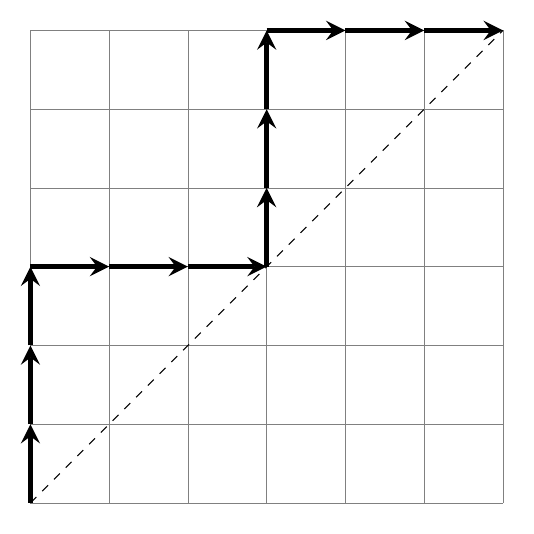
\begin{tikzpicture}
    %% 从 (0,0) 出发,长宽均为 6 ,1 为 上,0 为 右
    \NEpath{0,0}{6}{6}{1,1,1,0,0,0,1,1,1,0,0,0};
\end{tikzpicture}
\end{document}